\documentclass{../../slides-style}

\slidetitleext{Функциональное программирование на языке F\#}{16.02.2024}{Введение}

\begin{document}
    
    \begin{frame}[plain]
        \titlepage
    \end{frame}
    
    \section{Введение}
    
    \begin{frame}
        \frametitle{О чём этот курс}
        \begin{itemize}
            \item Теория и практика функционального программирования
            \begin{itemize}
                \item $\lambda$-исчисление
                \item Базовые принципы ФП (программирование без состояний, функции высших порядков, каррирование~и~т.д.)
                \item Типы в функциональном программировании (немутабельные коллекции,
                    генерики, автообобщение~и~т.д.)
                \item Паттерны функционального программирования (CPS, монады, point-free)
            \end{itemize}
            \item Программирование на F\# 
            \begin{itemize}
                \item ООП в F\#
                \item Асинхронное и многопоточное программирование в F\#
                \item Компиляторы
                \item Может, ещё про анализ данных и машинное обучение
            \end{itemize}
        \end{itemize}
    \end{frame}

    \begin{frame}
        \frametitle{Отчётность}
        \begin{itemize}
            \item Домашка (много несложной)
            \item Одна контрольная в середине семестра
            \item Доклад
            \item Сдача и учёт через HwProj 2
            \begin{itemize}
                \item \url{https://hwproj.ru/courses/20017}
            \end{itemize}
        \end{itemize}
    \end{frame}

    \begin{frame}
        \frametitle{Критерии оценивания}
        \begin{itemize}
            \item Как в прошлом семестре, ECTS
            \item Баллы за домашние задачи, баллы за контрольную
            \item Общий балл за домашки: $MAX(0, (n/N – 0.6)) * 2.5 * 100$
            \item Общий балл за контрольные: $n/N * 100$
            \item Итоговая оценка: минимум из этих двух баллов
            \item Дедлайны по домашкам, -1 балл за каждую неделю после дедлайна
            \item Сгорает не более половины баллов
            \begin{itemize}
                \item Таким образом, задачи на 1 балл не штрафуются вовсе
                \item Но их сделать проще, чем не сделать
            \end{itemize}
        \end{itemize}
    \end{frame}

    \begin{frame}
        \frametitle{Ориентировочно}
        \begin{itemize}
            \item Всего около 36 баллов за д/з и 10 за к/р
            \item A --- 35 балла за домашки, 9 за контрольную
            \item B --- 34 баллов за домашки, 8 за контрольную
            \item C --- 32 баллов за домашки, 7 за контрольную
            \item D --- 31 баллов за домашки, 6 за контрольную
            \item E --- 29 баллов за домашки, 5 за контрольную
        \end{itemize}
        
        \vspace{0.5cm}

        \begin{itemize}
            \item Разбалловка может измениться!
            \item Нагрузка правда меньше, делайте хорошие практики
        \end{itemize}
    \end{frame}

    \section{Введение в функциональное программирование}
    
    \begin{frame}
        \frametitle{Императивное программирование}
        Программа как последовательность \textbf{операторов}, изменяющих \textbf{состояние} вычислителя.

        Для конечных программ есть \textbf{начальное состояние}, \textbf{конечное состояние} и последовательность переходов:
        $$\sigma = \sigma_1 \rightarrow \sigma_2 \rightarrow ... \rightarrow \sigma_n = \sigma'$$
        
        Основные понятия:
        \begin{itemize}
            \item Переменная
            \item Присваивание
            \item Поток управления
            \begin{itemize}
                \item Последовательное исполнение
                \item Ветвления
                \item Циклы
            \end{itemize}
        \end{itemize}
    \end{frame}
    
    \begin{frame}
        \frametitle{Функциональное программирование}
        Программа как вычисление значения \textbf{выражения} в математическом смысле на некоторых входных данных.
        $$\sigma' = f(\sigma)$$
    
        \begin{itemize}
            \item Нет состояния $\Rightarrow$ нет переменных
            \item Нет переменных $\Rightarrow$ нет циклов
            \item Нет явной спецификации потока управления
        \end{itemize}
        Порядок вычислений не важен, потому что нет состояния, результат вычисления зависит только от входных данных.
    \end{frame}
    
    \begin{frame}[fragile]
        \frametitle{Сравним}
        \begin{alertblock}{C++}
            \begin{minted}{cpp}
int factorial(int n) {
    int result = 1;
    for (int i = 1; i <= n; ++i) {
        result *= i;
    }
    return result;
}
            \end{minted}
        \end{alertblock}
        \begin{exampleblock}{F\#}
            \begin{minted}{fsharp}
let rec factorial x =
    if x = 1 then 1 else x * factorial (x - 1)
            \end{minted}
        \end{exampleblock}
    \end{frame}

    \begin{frame}[fragile]
        \frametitle{Как с этим жить}
        \begin{itemize}
            \item Состояние и переменные \enquote{эмулируются} параметрами функций
            \item Циклы \enquote{эмулируются} рекурсией
            \item Последовательность вычислений --- рекурсия + параметры
        \end{itemize}
        \begin{exampleblock}{F\#}
            \begin{minted}{fsharp}
let rec sumFirst3 ls acc i =
    if i = 3 then 
         acc 
    else 
        sumFirst3 
            (List.tail ls) 
            (acc + ls.Head) 
            (i + 1)
            \end{minted}
        \end{exampleblock}
    \end{frame}

    \begin{frame}
        \frametitle{Зачем}
        \begin{itemize}
            \item Строгая математическая основа
            \item Семантика программ более естественна
            \begin{itemize}
                \item Применима математическая интуиция
            \end{itemize}
            \item Программы проще для анализа
            \begin{itemize}
                \item Автоматический вывод типов
                \item Оптимизации
                \item Строгая типизация
            \end{itemize}
            \item Более декларативно
            \begin{itemize}
                \item Ленивость
                \item Распараллеливание
            \end{itemize}
            \item Модульность и переиспользуемость
            \item Программы более выразительны
        \end{itemize}
    \end{frame}
    
    \begin{frame}[fragile]
        \frametitle{Пример: функции высших порядков}
        \begin{minted}{fsharp}
let rec sumFirst3 ls acc i =
    if i = 3 then acc 
    else sumFirst3 (List.tail ls) (acc + ls.Head) (i + 1)
        \end{minted}
        $$\Downarrow$$
        \begin{minted}{fsharp}
let sumFirst3 ls = 
    Seq.fold (fun x acc -> acc + x) 0 (Seq.take 3 ls)
        \end{minted}
        $$\Downarrow$$
        \begin{minted}{fsharp}
let sumFirst3 ls = ls |> Seq.take 3 |> Seq.fold (+) 0
        \end{minted}
        $$\Downarrow$$
        \begin{minted}{fsharp}
let sumFirst3 = Seq.take 3 >> Seq.sum
        \end{minted}
    \end{frame}

    \begin{frame}[fragile]
        \frametitle{Ещё пример}
        \framesubtitle{Возвести в квадрат и сложить все чётные числа в списке}
        \begin{minted}{fsharp}
let calculate = 
    Seq.filter (fun x -> x % 2 = 0) 
    >> Seq.map (fun x -> x * x) 
    >> Seq.reduce (+)
        \end{minted}
    \end{frame}

    \begin{frame}
        \frametitle{Почему тогда все не пишут функционально}
        \begin{itemize}
            \item Чистые функции не могут оказывать влияние на внешний мир. Ввод-вывод, работа с данными,
                    вообще выполнение каких-либо действий не укладывается в функциональную модель.
            \item Сложно анализировать производительность, иногда функциональные программы проигрывают
                    в производительности императивным. <<Железо>>, грубо говоря, представляет собой 
                    реализацию машины Тьюринга, тогда как функциональные программы определяются над
                    $\lambda$-исчислением.
            \item Требуется математический склад ума и вообще желание думать.
        \end{itemize}
    \end{frame}

    \section{F\#}

    \begin{frame}
        \frametitle{F\#}
        \begin{itemize}
            \item Типизированный функциональный язык для платформы .NET
            \item НЕ чисто функциональный (можно императивный стиль и ООП)
            \item Первый раз представлен публике в 2005 г., актуальная версия --- 8.0 (14 ноября 2023 года)
            \item Создавался под влиянием OCaml (практически диалект OCaml под .NET)
            \item Использует .NET CLI
            \item Компилируемый и интерпретируемый
            \item Иногда используется в промышленности, в отличие от многих чисто функциональных языков
        \end{itemize}
    \end{frame}

    \begin{frame}
        \frametitle{Что скачать и поставить}
        \begin{itemize}
            \item Visual Studio Community
            \item .NET 7 + Visual Studio Code + Ionide
            \item Прямо в браузере: \url{https://dotnetfiddle.net/}
            \item Rider
        \end{itemize}
    \end{frame}
    
    \begin{frame}[fragile]
        \frametitle{Пример программы}
        \begin{minted}{fsharp}
printfn "%s" "Hello, world!"
        \end{minted}
    \end{frame}

    \section{Let-определения}

    \begin{frame}[fragile]
        \frametitle{let-определение}
        \begin{minted}{fsharp}
let x = 1
let x = 2
printfn "%d" x
        \end{minted}
        можно читать как
        \begin{minted}{fsharp}
let x = 1 in let x = 2 in printfn "%d" x
        \end{minted}
        и понимать как подстановку $\lambda$-терма (про которые через одну пару)
    \end{frame}

    \begin{frame}[fragile]
        \frametitle{let-определение, функции}
        \begin{minted}{fsharp}
let powerOfFour x = 
    let xSquared = x * x
    xSquared * xSquared
        \end{minted}
        \begin{itemize}
            \item Позиционный синтаксис
            \begin{itemize}
                \item Отступы строго пробелами
                \item Не надо ";"
            \end{itemize}
            \item Нет особых синтаксических различий между переменной и функцией
            \item Не надо писать типы
            \item Не надо писать \textit{return}
        \end{itemize}
    \end{frame}

    \begin{frame}[fragile]
        \frametitle{Вложенные let-определения}
        \begin{minted}{fsharp}
let powerOfFourPlusTwoTimesSix n =
    let n3 =
        let n1 = n * n
        let n2 = n1 * n1
        n2 + 2
    let n4 = n3 * 6
    n4
        \end{minted}
        \begin{itemize}
            \item \textit{n3} --- не функция!
            \item Компилятор отличает значения и функции по наличию аргументов
            \item Значение вычисляется, когда до \textit{let} <<доходит управление>>, 
                    функция --- когда её вызовут. Хотя, конечно, функция --- тоже значение.
        \end{itemize}
    \end{frame}

    \section{Типы}

    \begin{frame}[fragile]
        \frametitle{Типы}
        \begin{minted}{fsharp}
let rec f x =
    if x = 1 then 
        1 
    else 
        x * f (x - 1)
        \end{minted}

        \begin{alertblock}{F\# Interactive}
            \begin{minted}{fsharp}
val f : x:int -> int
            \end{minted}
        \end{alertblock}
        Каждое значение имеет тип, известный во время компиляции
    \end{frame}

    \begin{frame}
        \frametitle{Элементарные типы}
        \begin{itemize}
            \item \textit{int}
            \item \textit{double}
            \item \textit{bool}
            \item \textit{string}
            \item ... (.NET)
            \item \textit{unit} --- тип из одного значения, (). Аналог void.
        \end{itemize}
    \end{frame}
    
    \begin{frame}[fragile]
        \frametitle{Кортежи (tuples)}
        \begin{minted}{fsharp}
let site1 = ("scholar.google.com", 10)
let site2 = ("citeseerx.ist.psu.edu", 5)
let site3 = ("scopus.com", 4)
let sites = (site1, site2, site3)

let url, relevance = site1
let site1, site2, site3 = sites
        \end{minted}
    \end{frame}

    \begin{frame}[fragile]
        \frametitle{Value Tuples}
        \begin{minted}{fsharp}
let origin = struct (0, 0)

let displace struct (x, y) struct (dx, dy)
    = struct (x + dx, y + dy)

displace origin struct (1, 1)
        \end{minted}
    \end{frame}

    \begin{frame}[fragile]
        \frametitle{Лямбды}
        \begin{minted}{fsharp}
let primes = [2; 3; 5; 7]
let primeCubes = List.map (fun n -> n * n * n) primes
        \end{minted}
        \begin{alertblock}{F\# Interactive}
            \begin{minted}{fsharp}
> primeCubes;;
val it : int list = [8; 27; 125; 343]
            \end{minted}
        \end{alertblock}
        \begin{minted}{fsharp}
let f = fun x -> x * x
let n = f 4
        \end{minted}
    \end{frame}

    \begin{frame}
        \frametitle{Списки}
        \begin{small}
            \begin{tabu} {| X[0.9 l p] | X[1 l p] | X[1 l p] |}
                \tabucline-
                Синтаксис                               & Описание                  & Пример                                      \\
                \tabucline-
                \everyrow{\tabucline-}
                $[]$                                    & Пустой список             & $[]$                                        \\
                $[expr; ...; expr]$                     & Список с элементами       & $[1; 2; 3]$                                 \\
                $expr :: list$                          & cons, добавление в голову & $1 :: [2; 3]$                               \\
                $[expr\ ..\ expr]$                      & Промежуток целых чисел    & $[1 .. 10]$                                 \\
                $[for\ x\ in\ list\ \rightarrow\ expr]$ & Генерированный список     & $[for\ x\ in\ 1..99\ \rightarrow\ x\ *\ x]$ \\
                $list\ @\ list$                         & Конкатенация              & $[1; 2]\ @\ [3; 4]$                         \\
            \end{tabu}
        \end{small}
    \end{frame}

    \begin{frame}[fragile]
        \frametitle{Примеры работы со списками}
        \begin{minted}{fsharp}
let oddPrimes = [3; 5; 7; 11]
let morePrimes = [13; 17]
let primes = 2 :: (oddPrimes @ morePrimes)
        \end{minted}
        \begin{minted}{fsharp}
let printFirst primes =
    match primes with
    | h :: t -> printfn "First prime in the list is %d" h
    | [] -> printfn "No primes found in the list"
        \end{minted}
    \end{frame}

    \begin{frame}[fragile]
        \frametitle{Устройство списков}
        \begin{center}
            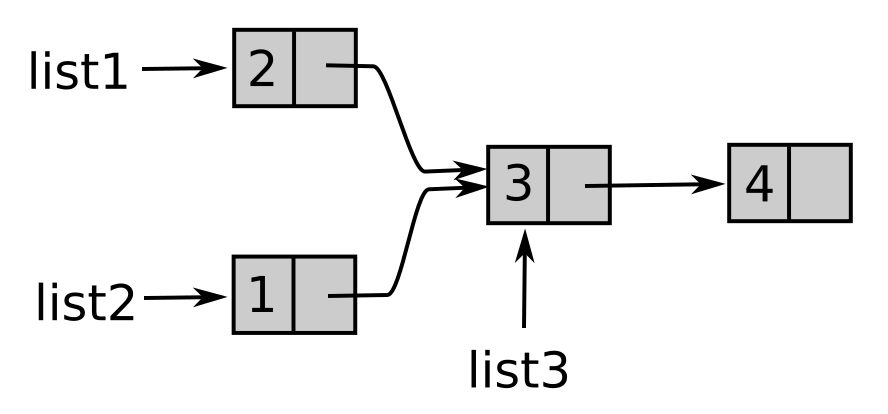
\includegraphics[width=0.4\textwidth]{lists.png}
        \end{center}
        \begin{minted}{fsharp}
let list3 = [3; 4]
let list1 = 2 :: list3
let list2 = 1 :: list3
        \end{minted}
        \begin{itemize}
            \item Списки немутабельны
            \item Cons-ячейки, указывающие друг на друга
            \item cons за константное время, @ --- за линейное
        \end{itemize}
    \end{frame}

    \begin{frame}
        \frametitle{Операции над списками}
        \framesubtitle{Модуль Microsoft.FSharp.Collections.List}
        \begin{small}
            \begin{tabu} {| X[0.5 l p] | X[1 l p] | X[1 l p] | X[0.5 l p] |}
                \tabucline-
                Функция                & Описание                            & Пример                                              & Результат            \\
                \tabucline-
                \everyrow{\tabucline-}
                List.length            & Длина списка                        & $List.length\ [1;2;3]$                              & $3$                  \\
                List.nth               & n-ый элемент списка                 & $List.nth\ [1; 2; 3]\ 1$                            & $2$                  \\
                List.init              & Генерирует список                   & $List.init\ 3 (fun\ i\ \rightarrow\ i * i)$         & $[0; 1; 4]$          \\
                List.head              & Голова списка                       & $List.head\ [1; 2; 3]$                              & $1$                  \\
                List.tail              & Хвост списка                        & $List.tail\ [1; 2; 3]$                              & $[2; 3]$             \\
                List.map               & Применяет функцию ко всем элементам & $List.map\ (fun\ i\ \rightarrow\ i * i)\ [1; 2; 3]$ & $[1; 4; 9]$          \\
                List.filter            & Отбирает нужные элементы            & $List.filter\ (fun\ x\ \rightarrow\ x\ \%\ 2 <> 0)\ [1; 2; 3]$ & $[1; 3]$  \\
                List.fold              & "Свёртка"  & $List.fold\ (fun\ x\ acc\ \rightarrow\ acc * x)\ 1\ [1; 2; 3]$               & $6$                  \\
            \end{tabu}
        \end{small}
    \end{frame}
    
    \begin{frame}[fragile]
        \frametitle{Тип Option}
        Либо \textit{Some что-то}, либо \textit{None}, представляет возможное отсутствие значения.
        \begin{minted}{fsharp}
let people = [ ("Adam", None); ("Eve" , None);
    ("Cain", Some("Adam","Eve"));
    ("Abel", Some("Adam","Eve")) ]
        \end{minted}
        \begin{minted}{fsharp}
let showParents (name, parents) =
    match parents with
    | Some(dad, mum) -> 
        printfn "%s, father %s, mother %s" name dad mum
    | None -> printfn "%s has no parents!" name
        \end{minted}
    \end{frame}

    \section{Функции}

    \begin{frame}[fragile]
        \frametitle{Рекурсия}
        \begin{minted}{fsharp}
let rec length l =
    match l with
    | [] -> 0
    | h :: t -> 1 + length t

let rec even n = (n = 0u) || odd(n - 1u)
and odd n = (n <> 0u) && even(n - 1u)
        \end{minted}
    \end{frame}

\end{document}
